\section{Part II: Quantum Circuits on Hardware}\label{sec:part2}

\subsection{Design}

Part~II moves the question to a physical substrate. I took four circuit pairs (\texttt{mod5\_4}, \texttt{tof\_3}, \texttt{barenco\_tof\_3}, \texttt{mod\_mult\_55}) from the Amy--Maslov--Nam benchmark family~\cite{amy2014tpar,nam2018automated}. Each pair implements one unitary twice: the standard baseline and a ZX-rewritten optimized circuit. ZX reduction machine-verifies pair equality before shipping (all four PASS), and \texttt{verify.py} re-verifies it independently from the committed QASM (Table~\ref{tab:pairs}). The record here is the compilation history: the rewrite proof that certifies the optimized circuit \emph{is} the same computation. I registered the predictions before any hardware ran, under a 1\% two-qubit depolarizing model, in size order: \texttt{mod5\_4} $+0.048$ $>$ \texttt{mod\_mult\_55} $+0.029$ $>$ \texttt{barenco\_tof\_3} $+0.020$ $>$ \texttt{tof\_3} $+0.013$ (near-parity control). Execution as registered: both arms interleaved in one job per pair, 8192 shots per arm, optimization level 1, \texttt{seed\_transpiler\,=\,7}, IBM \texttt{ibm\_fez}, 2026-07-18~\cite{javadi2024qiskit}. A noiseless simulator check ran first (both arms fidelity 1.0, delta zero), so any gap on the chip is hardware, not a compile error. One note on the metric: all four circuits have deterministic ideal outputs, a single bitstring, so ``fidelity'' here means the probability of measuring the exact correct answer. The layout pass placed all four pairs on overlapping low-error subsets in the qubit 117 to 145 region (mean CZ error $1.85$ to $2.11\times10^{-3}$ on the edges used, below that day's median).

\begin{table}[htbp]
\centering\small
\caption{Certified pairs, pre-transpile counts (baseline $\to$ optimized). Verification: ZX reduction of the composed pair to the identity. \emph{Source: project data~\cite{appliedrepo2026}.}}
\label{tab:pairs}
\begin{tabular}{lccccc}
\toprule
circuit & qubits & 2q gates & T-count & depth & verified \\
\midrule
\texttt{mod5\_4} & 5 & $28 \to 20$ & $28 \to 8$ & $48 \to 20$ & PASS \\
\texttt{tof\_3} & 5 & $18 \to 16$ & $21 \to 15$ & $31 \to 30$ & PASS \\
\texttt{barenco\_tof\_3} & 5 & $24 \to 22$ & $28 \to 16$ & $42 \to 43$ & PASS \\
\texttt{mod\_mult\_55} & 9 & $48 \to 42$ & $49 \to 35$ & $51 \to 46$ & PASS \\
\bottomrule
\end{tabular}
\end{table}

\subsection{Results}

\begin{table}[htbp]
\centering\small
\caption{Part II main results, IBM \texttt{ibm\_fez}, 2026-07-18. $z$ from per-shot paired statistics; transpiled counts are post-layout. \emph{Source: project data~\cite{appliedrepo2026}.}}
\label{tab:part2}
\begin{tabular}{lccccc}
\toprule
pair & $\Delta$ observed & $z$ & $\Delta$ predicted & transpiled 2q (b$\to$o) & depth (b$\to$o) \\
\midrule
\texttt{mod\_mult\_55} & $+0.0670$ & $+9.5$ & $+0.029$ & $99 \to 117$ & $217 \to 204$ \\
\texttt{mod5\_4} & $+0.0248$ & $+4.8$ & $+0.048$ & $52 \to 38$ & $206 \to 95$ \\
\texttt{barenco\_tof\_3} & $+0.0167$ & $+3.9$ & $+0.020$ & $42 \to 34$ & $164 \to 126$ \\
\texttt{tof\_3} (control) & $-0.0042$ & $-1.1$ & $+0.013$ & $30 \to 28$ & $118 \to 112$ \\
\bottomrule
\end{tabular}
\end{table}

Two verdicts, per the registered decision tree. \emph{Direction: confirmed} on all three effect pairs. The control landed at $-0.004$, within shot noise of zero, which rules out a systematic interleaved-arm bias. \emph{Ordering: falsified}, and stated as falsified. The registered ladder put \texttt{mod5\_4} first and \texttt{mod\_mult\_55} second; observation inverted them. The 9-qubit circuit won by the largest margin despite carrying \emph{more} transpiled two-qubit gates than its baseline (117 vs.\ 99). It won through depth (204 vs.\ 217): on a real device, coherence time prices circuits alongside gate error, so a one-parameter depolarizing model cannot rank them. Compilation pays on hardware; the simulator's ordering does not transfer.

\begin{figure}[htbp]
\centering
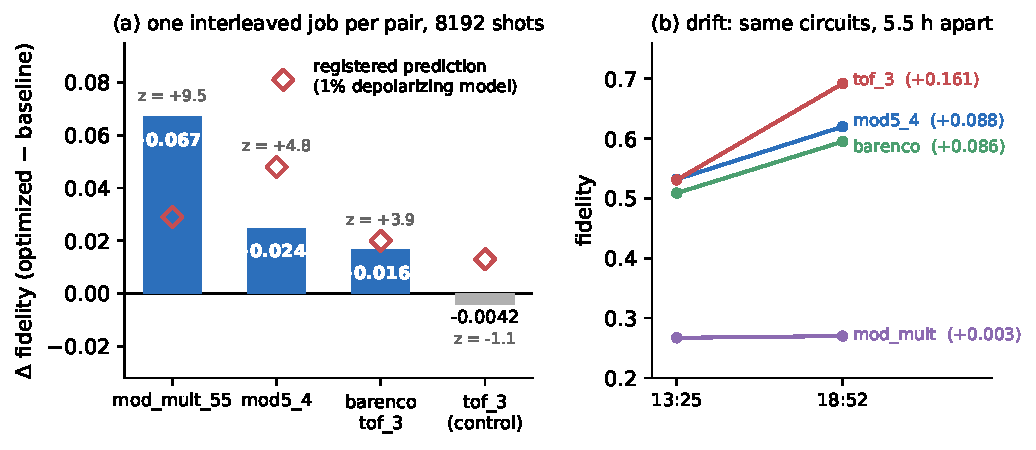
\includegraphics[width=0.92\textwidth]{figs/f3_part2_deltas.pdf}
\caption{Part II results in two panels. (a) Observed deltas against the registered predictions, one interleaved job per pair, 8192 shots, IBM \texttt{ibm\_fez}, 2026-07-18. (b) The drift measurement behind the interleaving rule: identical circuits in identical no-DD condition, re-measured hours later, move by up to $+0.161$. \emph{Source: figure created by the author from project data~\cite{appliedrepo2026}.}}
\label{fig:part2}
\end{figure}

\subsection{Error budget against the device ceiling}

After the verdict (not pre-registered), I compared each arm against its ceiling from that day's recovered calibration: $\prod(1-\varepsilon_{\mathrm{CZ}})$ over the exact edges used, times $\prod(1-\varepsilon_{\mathrm{ro}})$ over the exact qubits measured (Table~\ref{tab:ceilinghw}). Seven of eight arms sit at 99\% to 104\% of ceiling: the runs saturate the unmitigated hardware limit, so the deltas are close to a pure compilation effect. The one sub-ceiling arm, the \texttt{mod\_mult\_55} baseline at 89\%, carries about eight points of error the gate-count model cannot explain, while its optimized arm on mostly the same qubits sits at 103\%. The excess tracks circuit duration, independently supporting the duration reading. Above-ceiling values are physical: randomized benchmarking counts all Pauli errors~\cite{magesan2012rb}, but Z-type errors near measurement do not change a computational-basis output, so the RB ceiling is mildly conservative for this family.

\begin{table}[htbp]
\centering\small
\caption{Error budget vs.\ execution-time calibration (recovered from the four jobs' backend properties). Above-ceiling values are physical for this circuit family (see text). \emph{Source: project data~\cite{appliedrepo2026}.}}
\label{tab:ceilinghw}
\begin{tabular}{llccc}
\toprule
pair & arm & ceiling & measured & \% of ceiling \\
\midrule
\texttt{mod5\_4} & baseline & 0.875 & 0.865 & 99\% \\
\texttt{mod5\_4} & optimized & 0.902 & 0.890 & 99\% \\
\texttt{tof\_3} & baseline & 0.908 & 0.941 & 104\% \\
\texttt{tof\_3} & optimized & 0.913 & 0.937 & 103\% \\
\texttt{barenco\_tof\_3} & baseline & 0.892 & 0.912 & 102\% \\
\texttt{barenco\_tof\_3} & optimized & 0.907 & 0.928 & 102\% \\
\texttt{mod\_mult\_55} & baseline & 0.758 & 0.678 & \textbf{89\%} \\
\texttt{mod\_mult\_55} & optimized & 0.726 & 0.745 & 103\% \\
\bottomrule
\end{tabular}
\end{table}

One further covariate qualifies the registered number. A transpile-seed sweep (20 seeds, level 1, Fez snapshot) shows seed~7 gave the \texttt{mod\_mult\_55} optimized arm its \emph{worst} routing of all twenty (117 2q; sweep minimum 102, median 112.5), while the baseline drew near-best routing (99; minimum 96). The registered $+0.067$ was therefore measured with the optimized arm at its worst draw, and is plausibly a lower bound on the compilation effect at this site.

\subsection{Replication, routing decomposition, and drift}

Six days later I re-ran the flagship pair under stricter control (R2$'$): both arms pinned to one shared nine-qubit layout, one interleaved job. Baseline 99 2q at fidelity 0.639; optimized 102 2q at 0.700. The delta, $+0.0604$ against the registered $+0.0670$, shows the compilation gain replicates at matched placement. A third arm on identical qubits with deliberately worse routing (114 2q) measured 0.565: a routing effect of $-0.1346$ for 12 extra two-qubit gates and 18 extra depth. With that day's calibration (mean CZ $5.38\times10^{-3}$ vs.\ $4.63\times10^{-3}$ on the good edges), the ceiling model explains 0.077 of the 0.135 drop: 57\%, the corrected figure, superseding an earlier informal 5$\times$ estimate that used the wrong CZ error. The remaining $\approx 0.058$ tracks depth. Routing skill matters, but depth has its own measurable price.

The device state that day is part of the record: CZ errors on these qubits ran $4.48$ to $5.38\times10^{-3}$, more than double the $2.11\times10^{-3}$ of 2026-07-18, and all three arms beat their ceilings (107\%, 121\%, 112\%), consistent with RB conservatism for computational-basis outputs.

The drift measurement justifies the interleaving rule. Same circuits, same no-DD condition, two jobs 5.5 hours apart: \texttt{mod5\_4} $0.532 \to 0.620$; \texttt{tof\_3} $0.531 \to 0.692$; \texttt{barenco} $0.509 \to 0.595$; \texttt{mod\_mult} $0.267 \to 0.270$. That is up to $+0.161$ in an afternoon, and $+0.03$ to $+0.08$ in the 32 minutes between two consecutive jobs. These swings exceed most effects measured in this project, including the registered $+0.067$. Any cross-job comparison in this work is therefore uninterpretable, which is why the cross-job DD comparison (R1) is invalid as executed.

\subsection{The mirror protocol, dynamical decoupling, and two rejected explanations}

The mirror experiment makes the hardware itself check the equality witnesses. For each registered pair $p$, a \emph{true mirror} runs $X(x)\cdot B_p \cdot O_p^{-1}$ on a random input basis state $|x\rangle$ (seeded, recorded), with barriers so the transpiler cannot cancel the halves; if $B_p \equiv O_p$ the composition returns exactly $x$. A \emph{deranged mirror} runs $X(x)\cdot B_p \cdot O_q^{-1}$ with $q \neq p$, and $x$ is redrawn until the ideal output differs from $x$, which guards against inputs that happen to be fixed points of the composition. The metric is the return probability $r = P(\text{measure exactly } x)$ at 8192 shots, all circuits in one interleaved job. Registered predictions: M1, every true mirror returns $r \geq 0.25$ and beats its deranged partner by 0.3; M2, point predictions from the product of the per-arm fidelities ($\pm 0.15$); M3, every deranged mirror stays at $r \leq 0.15$. One honest design note belongs in the record: the first draft placed a random Pauli layer at the joint, which is wrong for non-Clifford circuits (the layer conjugates through $B$, so the expected string would need simulation, defeating the protocol). Randomized inputs give the same protection with a simulation-free expectation; the correction was logged before submission.

Results. True mirrors returned 0.267 to 0.692; deranged mirrors 0.0002 to 0.086. M3 confirmed; the derangement control works. The M2 point predictions failed low on all four pairs. Two hypotheses were registered to explain the undershoot: idle dephasing (suppressing it should raise true-mirror returns) and metric blindness (per-arm fidelity is scored on computational-basis histograms, blind to the phase errors a mirror exposes through $O^{-1}$).

The first test of idle dephasing (R1) compared separate jobs five hours apart and is confounded by drift; Section~\ref{sec:errors} owns that design error in full, and its recorded verdicts (R1a/b failed, R1c confirmed) stand as measured but isolate nothing.

The corrected rerun (R1$'$) put all sixteen circuits, eight mirrors times \{no-DD, DD\}, in one job, with DD as an XX sequence of native X pulses. Result: uniformly harmful. Paired deltas $-0.076$, $-0.022$, $-0.005$, $-0.039$, mean $-0.036$. Deranged mirrors stayed under 0.15 as registered (max 0.070), so DD did not manufacture signal. The added pulses, 80 to 225 per circuit, cost more error than the idle dephasing they suppress at this scale. Per the falsification clause, the idle-dephasing explanation is \textbf{rejected}. The metric-blindness hypothesis remains \textbf{untested} by any run so far, and I label it as such rather than carry it quietly. One data-integrity caveat: DD pads idle qubits across the full 156-qubit register, so the extraction step counts every qubit and the recorded DD-arm ceilings collapse to 0.039. They are artifacts; only the no-DD ceilings are used.

\subsection{Two design errors, owned}\label{sec:errors}

\paragraph{Cross-job DD (R1).} The first DD run compared a DD job at 13:25 against a no-DD job at 18:20: five hours of device drift confounded with the treatment, in direct violation of this project's own interleaving protocol. Its measured deltas were mixed in sign (\texttt{mod5\_4} $-0.033$, \texttt{tof\_3} $+0.089$, \texttt{barenco} $+0.055$, \texttt{mod\_mult\_55} $-0.115$; mean $-0.001$; deranged max 0.086), so R1a/b failed and R1c confirmed, and the recorded verdicts stand as measured. But the run does not isolate a DD effect; two of its four sign readings were later shown to be drift. R1$'$ is the corrected measurement.

\paragraph{Seed changes layout (R2).} The seed-11 rerun treated \texttt{seed\_transpiler} as a routing knob. It is not: the seed changes the layout, and the two arms landed on disjoint physical qubits (0/9 overlap, versus 7/9 in the registered runs). Its $+0.171$ delta therefore compared two different qubit sets and is not comparable to the registered $+0.067$. R2$'$ is the corrected measurement, and the seed sweep that exposed the error is committed alongside it.
